\chapter{Compilation}
\label{chp:compilation}
% TODO: PISA cite
The following chapter will present the design for the reversible heap manager and the translation schemes used in the process of translating \rooplpp to the reversible low-level machine language \textsc{PISA}.

\section{Dynamic Memory Management}
\label{sec:dynamic-memory-management}
Native support of complex data structures is not a trivial matter to implement in a reversible computing environment. Variable-sized records and frames need to be stored efficiently in a structured heap, while avoiding garbage build-up to maintain reversibility. A reversible heap manager layout has been proposed for a simplified version of the reversible functional language \textsc{RFun} and later expanded to allow references to avoid deep copying values~\cite{ha:heap, ty:rfun, tm:refcounting}.

The following section presents a discussion of various heap manager layouts along with their advantages and disadvantages in terms of implementation difficulty, garbage build-up and the OOP domain. 

\subsection{Fragmentation}
\label{subsec-fragmentation}
An important matter to consider when designing a heap layout for dynamic memory allocation is efficient memory usage. In a stack allocating memory layout, the stack discipline is in effect, meaning only the most recently allocated data can be freed. This is not the case with heap allocation, where data can be freed regardless of allocation order. This feature comes with the consequence of potential memory fragmentation, as blocks are being freed in any order~\cite{tm:languages}.

We distinguish different types of fragmentation as internal or external fragmentation.

\subsubsection{Internal Fragmentation}
Internal fragmentation occurs in the memory heap when part of an allocated memory block is unused. This type of fragmentation can arise from a number of different scenarios, but mostly it originates from \textit{over-allocating}. 

An example of \textit{over-allocating} would be a scenario where we are allocating memory for an object of size $m$ onto a simple, fixed-sized block heap, where the fixed block size is $n$ and $m \neq n$. If $n > m$, internal fragmentation would occur of size $n-m$ for every object of size $m$ allocated in said heap. If $n < m$, numerous blocks would be required for allocation to fit our object. In this case the internal fragmentation would be of size $m + n - (m + n) \mod n$ per allocated object of size $m$. 

\begin{figure}[ht]
\centering
\texttt{TODO}
\caption{Example of internal fragmentation due to \textit{over-allocation}}
\label{fig:internal-frag-example}
\end{figure}

Figure~\ref{fig:internal-frag-example} visualizes the examples of internal fragmentation build-up from \textit{over-allocating} memory. 

Intuitively, internal fragmentation can be prevented by ensuring that the size of the block(s) being used for allocating space for an object of size $m$ either match or sums to this exact size.

\subsubsection{External Fragmentation}
External fragmentation materializes in the memory heap when a freed block becomes partly or completely unusable for future allocation if it, say, is surrounded by allocated blocks but the size of the freed block is too small to contain any object on its own.

This type of fragmentation is generally a more substantial cause of problems than internal fragmentation, as the size of external fragmentation blocks usually are larger than the ones created from internal fragmentation, depending on the heap implementation (In a layout using variable-sized blocks of, say, size $2^n$, the internal fragment size becomes considerable for large $n$s). 

Non-allocatable external fragments become a problem when there it is impossible to allocate space for a large object as a result of too many non-consecutive blocks scattered around the heap, caused by the external fragmentation. Physically, there is enough space to store the object, but not in the current heap state. In this scenario we would need a garbage collector to clean the heap and relocate blocks in such a manner that the fragmentation disperses.

\begin{figure}[ht]
\centering
\texttt{TODO}
\caption{Example of external fragmentation}
\label{fig:external-frag-example}
\end{figure}

\subsubsection{Consequences of Fragmentation in the Reversible Setting}
Fragmentation management and handling is particularly interesting within in the reversible setting. As reversible programmers we strive to maintain an \textit{exact} (or equivalent) computational state during program execution, such that we at any time can reverse the computational direction and return the a previous state. If external memory fragmentation is left unchecked in a reversible dynamic memory allocation implementation, we can easily run into the following scenario

\begin{itemize}
\item Object $A$, $B$ and $C$ are allocated on the heap in that order. The size of $A$ is one block of memory, $B$' size is two blocks and $C$'s size is three blocks.
\item $B$ is freed, leaving external fragmentation of two blocks in between $A$ and $C$.
\item $C$ is freed, thus leaving a total of five blocks of freed memory after $A$.
\item The computational direction is reverted and we now allocate $C$ again, which is allocated in the first three blocks next to $A$.
\item $B$ is then allocated again, thus giving us the order $A-C-B$ instead of the original $A-B-C$ order.
\end{itemize}  

Figure~\ref{fig:external-frag-comp-state-conseq} shows this exact scenario.

\begin{figure}[ht]
\centering
\texttt{TODO}
\caption{Potential state-changing side effect of external fragmentation in the reversible setting}
\label{fig:external-frag-comp-state-conseq}
\end{figure}

Furthermore, it is in our interest to limit external fragmentation as removing it during program execution would require a garbage collector, which is a non-trivial matter to implement. \citeauthor{tm:garbage} presented a heap manager for reversible functional languages using reference counts and hashing to achieve garbage collection in \cite{tm:garbage}, but it is not immediately clear how this garbage collection could translate to an object-oriented language.

\subsection{Memory Garbage}
\label{subsec-memory-garbage}
Traditionally, freed memory blocks are simply re-added to the free-list during deallocation and no modification of the actual data stored in the block is done. In the reversible setting we must return the memory block to the original state the block was in before the allocation occurred (e.g. zero-cleared registers), to uphold the time-invertible and two-directional computational model. 

Thus, in the reversible setting it should be our goal to also return the memory to its original state after program termination. With heap allocation, we will need one or more free-lists to keep track of free blocks during program execution, which must be stored in memory, besides the actual heap representation. These free-lists can essentially be considered garbage and as such, they must also be returned to their original state after execution. Furthermore, the if the heap grows during execution, it should be returned to its original size.

Returning the free-list(s) to their original states is a non-trivial matter, depending on the heap layout. \citeauthor{ha:heap} introduced heap allocation and deallocation, but without restoring the free-list to its original state in~\cite{ha:heap}. The argument for not restoring the free-list is that it can be considered harmless garbage in the sense that the free-list left after termination is equivalent, as it contains the same blocks, but linked in a different order, depending on the allocation and deallocation order during program execution.

This intuitively leads to the question of garbage classification. In the reversible setting all functions are injective. Thus, given some $input_f$, the injective function $f$ produces some $output_f$ and some $garbage_f$ (e.g. storing data in the heap, so the free list changes, the heap grows, etc.). Its inverse function $f^{-1}$ must thus take $f$'s $output_f$ and $garbage_f$ as $input_{f^{-1}}$ to produce its output $output_{f^{-1}}$ which is $f$'s $input_f$. However, in the context of reversible heaps, we must consider all free-lists as of "equivalent garbage class" and thus freely substitutable with each other, as injective functions still can drastically change the block layout, free-list order, etc. during its execution in either direction. Figure~\ref{fig:equivalent-free-lists} shows how any free-list can be passed between a function $f$ and its inverse $f^{-1}$. 

\begin{figure}[ht]
\centering
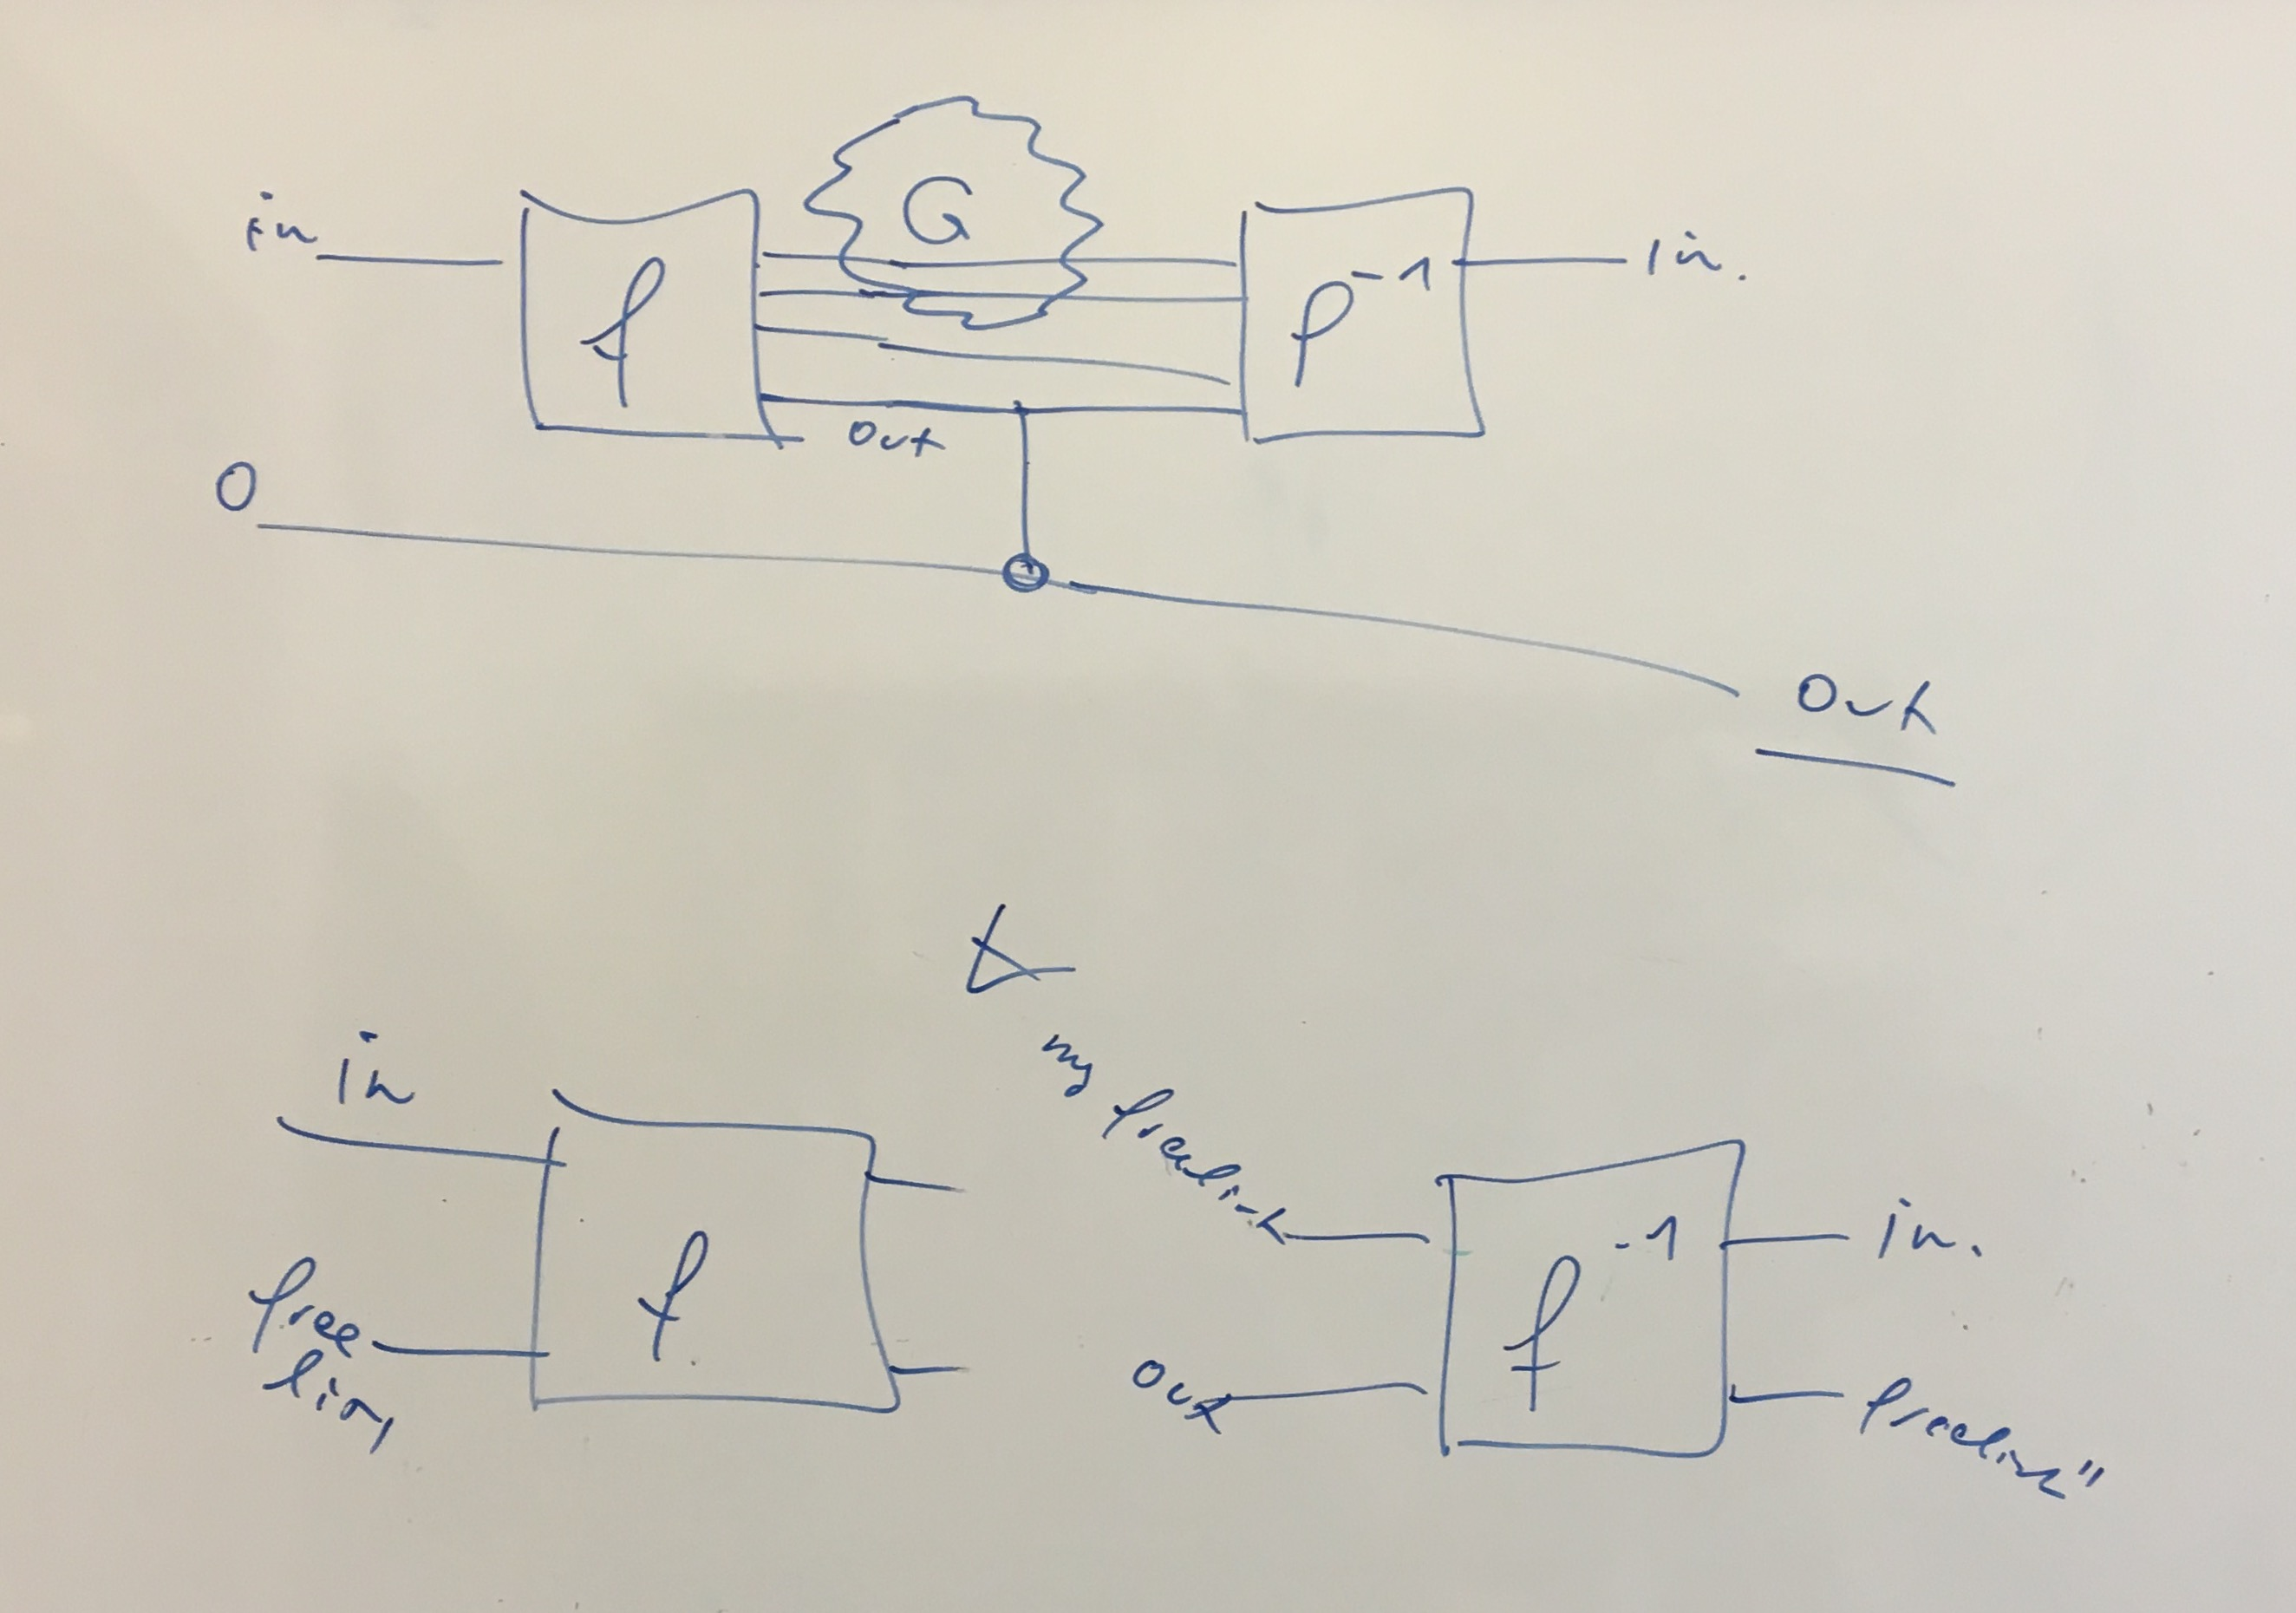
\includegraphics[width=0.7\textwidth]{garbage-classes}
\caption{All free-lists are considered equivalent in terms of injective functions (Temporary photo)}
\label{fig:equivalent-free-lists}
\end{figure}


\subsection{Heap manager layouts}
\label{subsec-heap-manager-layout}
Heap managers can be implemented in numerous ways. Different layouts yield advantages when allocating memory, finding a free block or when collecting garbage. As our goal is to construct a garbage-free heap manager, our finalized design should emphasize and reflect this objective in particular. Furthermore, we should attempt to allocate and deallocate memory as efficiently as possible, as merging and splitting of blocks is a non-trivial problem in a reversible setting.

For the sake of simplicity, we will not consider the the issue of retrieving memory pages reversibly. A reversible operating system is a long-term dream of the reversible programmer and as reversible programming language designers, we assume that \rooplpp will be running in a  environment, in which the operating system will be supplying memory pages and their mappings. As such, the following heap memory designs reflect this preliminary assumption, that we always can query the operating system for more memory. 

Historically, most object-oriented programming languages utilize a dynamic memory manager during program execution. In older, lower-level languages such as \textsc{C}, memory allocation had to be stated explicitly and with the requested size through the \texttt{malloc} statement and deallocated using the \texttt{free} statement. Modern languages, such as \textsc{C\texttt{++}}, \textsc{Java} and \textsc{Python}, \textit{automagically} allocates and frees space for objects and variable-sized arrays by utilizing their dynamic memory manager to dispatch \texttt{malloc}- and \texttt{free}-like operations to the operating system and managing the obtained memory blocks in private heap(s)~\cite{wh:cpp_memory, bv:jvm, py:memory}. The heap layout of these managers vary from language to language and compiler to compiler.

% Reversible Heaps
Previous work on reversible heap manipulation has been done for reversible functional languages in~\cite{ha:heap, jsk:translation, tm:garbage}.

% TODO: Something about Cons/Nil heap
\texttt{TODO: Something about Cons/Nil heap from~\cite{ha:heap}}

% TODO: Modifications to said 
\texttt{TODO: Something about ref count extension~\cite{tm:refcounting}}

For the sake of simplicity in the following heap layout pseudo-code outlines, we assume access to the following subroutines (with parameter passing), inspired by the body of \citeauthor{ha:heap}'s \texttt{get\_free} subroutine.

In order to reversibly allocate a block, we assume access to the subroutine \texttt{allocate\_block} which, given the register $r_{cell}$ where we want the address of the allocated block stored and the register $r_{flp}$ containing the free-list pointer, effectively pops the head of the free-list to  $r_{cell}$. Listing~\ref{lst:allocate-block-sub} shows the subroutine.

\begin{lstlisting}[caption={\texttt{allocate\_block} subroutine}, language=janus, style=basic,label={lst:allocate-block-sub}]
procedure allocate_block($r_{cell}$, $r_{flp}$)
	EXCH $r_{cell}$ $r_{flp}$
	SWAP $r_{cell}$ $r_{flp}$
\end{lstlisting}

In order to grow the heap, we assume access to the subroutine \texttt{grow\_heap} which, given the register $r_{hp}$ containing the heap pointer and a number $n$ specifying how much the heap should grow, increments the heap pointer by $n$. Listing~\ref{lst:grow-heap-sub} shows the subroutine.

\begin{lstlisting}[caption={\texttt{grow\_heap} subroutine}, language=janus, style=basic,label={lst:grow-heap-sub}]
procedure grow_heap($r_{hp}$, $n$)
	ADDI $r_{hp}$ $n$
\end{lstlisting}

Finally, in order to move the heap, we assume access to the subroutine \texttt{move\_heap} which, given the register $r_{hbp}$ containing a pointer to the \textit{bottom of a heap}\footnote{assuming it exists} and the register $r_{hp}$ containing the heap pointer and a number $n$ representing the amount the heap should be moved, iterates every memory address in the heap, starting at the top, and moves the memory block $n$ spaces. This is down using a top-down approach to avoid overwriting data. 

\begin{lstlisting}[caption={\texttt{move\_heap} subroutine}, language=janus, style=basic,label={lst:move-heap-sub}]
procedure move_heap($r_{hbp}$, $r_{hp}$, $n$, $m$)
	from  i = $r_{hp}$
    do
        SWAP $r_i$ $r_{i+n}$
        i -= 1 				; 1 word (?)
    until i = r_{hbp} - n
\end{lstlisting}


\subsubsection{Memory Pools}
A simple layout for a heap manager would allocate memory using fixed-size blocks regardless of the actual size of the record, which is known as memory pooling~\cite{bk:memorypool}. The advantage of a heap layout following this approach would lie in the simplicity of its implementation, as a simple linked list of identical-sized free cells would need to be maintained. If we assume a our fixed-sized blocks are of size $n$ machine words, the following \texttt{get\_free} subroutine allocates and deallocates memory cells for a record of size $m$.

\begin{lstlisting}[mathescape=true, caption={Allocating and deallocating records of size $m$ using block of a fixed size $n$. Code modified from~\cite{ha:heap}}, language=janus, style=basic,label={lst:memory-pool}]
if ($r_{flp}$ == 0) 
then
	XOR $r_{cell}$ $r_{hp}$
	call grow_heap($r_{hp}$, $m + n - (m + n)  \% n$)
else
	call allocate_block($r_{cell}$, $r_{flp}$)
fi ($r_{flp}$ == 0) && ($r_{cell}$ == $r_{hp}$ - ($m + n - (m + n)  \% n$))
\end{lstlisting}

Listing~\ref{lst:memory-pool} shows the modified \texttt{get\_free} subroutine for allocating and deallocating memory blocks in a memory pool layout. If the free-list is empty, the block which the heap pointer is currently pointing at is allocated and the heap is grown by $m + n - (m + n)  \% n$ blocks (rounding up to nearest number of blocks of size $n$ when allocating object of size $m$). If the free-list is non-empty, the \texttt{allocate\_block} subroutine is called.  

A huge disadvantage to using fixed-sized memory blocks is the external fragmentation that occurs when freeing blocks, if the program's objects are not of the same size. When freeing a number of blocks in the middle of a section of allocated blocks, external fragmentation occurs, which becomes a problem if we need to allocate space for a large record but only have small sections of fixed-blocks available, scattered throughout the heap. A garbage collector could solve this issue, but is a non-trivial matter to implement.

\texttt{TODO: Graphics}

\texttt{TODO: Present various layout using fixed-size blocks - Trees, continuous?}


\subsubsection{Buddy Memory}
In this approach we have all blocks be variable-size of the power-of-two. Having different block sizes and methods for splitting a larger block into smaller ones reduces fragmentation. In terms of implementation, reversible splitting and merging might be possible as we're always doubling the size when merging and halving when splitting, thus making the operations logically inverse of each other~\cite{dk:buddyalloc}.

We can reversibly and recursively split blocks using subroutine \texttt{split\_block}. The subroutine takes two registers $r_{cell1}$ and $r_{cell2}$ to contain the split block. If the passed register $r_{fpl}$ containing the free-list pointer of the heap for $2^{n+1}$ is empty, we recursively call the \texttt{split\_block}\footnote{Unsure if this works?}. If the free-list of the heap for $2^{n+1}$ heap is not empty, we pop the head of the free list into $r_{cell1}$ and split the block by setting the pointer halfway through the block in register $r_{cell2}$. Listing~\ref{lst:split-block-sub} shows the subroutine.   

\begin{lstlisting}[caption={\texttt{split\_block} subroutine}, language=janus, style=basic,label={lst:split-block-sub}]
procedure split_block($r_{cell1}$, $r_{cell2}$, $r_{fpl}$, $n$)
	if ($r_{flp}$ == 0) 
	then
		call split_block($r_{cell1}$, $r_{cell2}$, $r_{fpl}$, $n*2$)
	else
		EXCH $r_{cell1}$ $r_{flp}$
		SWAP $r_{cell1}$ $r_{flp}$
		EXCH $r_{cell2}$ $r_{cell1}$ + n / 2
	fi ($r_{flp}$ == 0)
\end{lstlisting}
\texttt{TODO: Consider Torben's suggesting with only merging/splitting if adjacent block}

Assuming we have access to an array of pointers $flps[]$, pointing to the beginning of a free list, index at its power-of-two and subroutine in Listing~\ref{lst:split-block-sub}, we could allocate and deallocate a record of size $n$ in a buddy memory layout reversibly in the following manner

\begin{lstlisting}[mathescape=true, caption={Allocating and deallocating records of size $n$ using Buddy Memory}, language=janus, style=basic]
maxPo2 = 2^10
from powerOfTwo = 2
do
	powerOfTwo = powerOfTwo * 2
until powerOfTwo < n
	
if (flps[powerOfTwo] == 0) 
then
	from nextPo2 = powerOfTwo * 2
	do
		call split_block($r_{cell}^{powerOfTwo}$, $r_{cell2}^{powerOfTwo}$, flps[nextPo2], nextPo2)
	until (nextPo2 > maxPo2)
	
	 if (flps[powerOfTwo] == 0)
	 then
	 	call grow_heap(r_{hp}^{maxPo2}, maxPo2)
		call split_block($r_{cell}^{powerOfTwo}$, $r_{cell2}^{powerOfTwo}$, flps[nextPo2], nextPo2)
	else
		EXCH flps[powerOfTwo] $r_{cell2}^{powerOfTwo}$
	fi (flps[powerOfTwo] == 0)
else
	call allocate_block($r_{cell}^{powerOfTwo}$, flps[powerOfTwo])
fi (flps[powerOfTwo] == 0) 
\end{lstlisting}
\texttt{TODO: Consider need\_max\_heap\_grow subroutine?}

The \texttt{get\_free} modification for a buddy memory layout starts by finding the $2^n$ heap which the record of size $n$ can fit it. Afterwards, if the free-list pointer for the found heap is empty, the \texttt{split\_block} subroutine is called to obtain two blocks of the given size. If no blocks can be found and split (recursively), the biggest $2^n$ heap is grown by one block and the then \texttt{split\_block} is called again (recursively) to obtain two blocks of the desired size. Once two blocks have been obtained, the first is used for allocating our object and the second is set as the head of the free list. In the case we the free list of the found heap is non-empty, we simply call the \texttt{allocate\_block} subroutine.

\texttt{TODO: Graphics}

\subsubsection{One heap per record type}
Another layout approach would be maintaining one heap per record type in the program. During compilation, classes would be analysed and a heap for each class would be created. The advantage of this approach would be less garbage generation, as each allocation is tailored as closely as possible to the size of the record obtained from a static analysis during compilation. The obvious disadvantage is the amount of book-keeping and workload associated with growing and shrinking a heap and its neighbours.

\texttt{Algorithm: Determine heap for record type, call get\_free on found heap}

\texttt{TODO: Graphics}

\subsubsection{Shared heap, record type-specific free lists}
A combination of the previous layouts would consist of a single heap, but record-specific free lists. This way, we ensure minimal fragmentation when allocating and freeing as the different free lists ensures that allocation of an object wastes as little memory as possible. By only keeping one heap, we eliminate the growth/shrinking issues of the multiple heap layout. There is, however, still a considerable amount of book-keeping involved in maintaining multiple free-lists. The bigger the number of unique classes defined in a program, the more free-lists we need to maintain during execution. If the free-lists are not allowed to point at the same free block (which they intuitively shouldn't in order to ensure reversibility), programs with many classes, say one hundred, could potentially fill up the heap with one hundred free lists, but only ever allocate objects for one of the classes, thus wasting a lot of memory on unused free lists. This scenario could potentially be avoided with compiler optimizations.

\texttt{Algorithm: Find block size for record type-specific free list, call get\_free on shared heap}

\texttt{TODO: Graphics}

\subsubsection{One heap per power-of-two}
A different approach as to having one heap per record type, would be having one heap per power-of-two until some arbitrary size. Using this approach, records would be stored in the heap which has a block size of a power-of-two closes matching to the record's size. This layout is a distinction from the "one heap per record type" as it still retains the size-optimized storing idiom but allows the heaps to contain records of mixed types. For programs with a large amount of small, simple classes needed to model some system, where each class is roughly the same size, the amount of heaps constructed would be substantially smaller than using one heap per record type, as many records will fit within the same heap. Implementation wise, the number of heaps can be determined at compile time. Furthermore, to ensure we do not end up with heaps of very large memory blocks, an arbitrary power-of-two size limit could be set at, say, 1 kb . If any record exceeds said limit, it could be split into $\sqrt{n}$ size chunks and stored in their respective heaps.\\
This approach does, however, also suffer from large amount of book-keeping and fiddling when shrinking and growing adjacent heaps.

\texttt{Algorithm: Similar to buddy memory?}

\texttt{TODO: Graphics}

\begin{figure}[H]
  \centering
  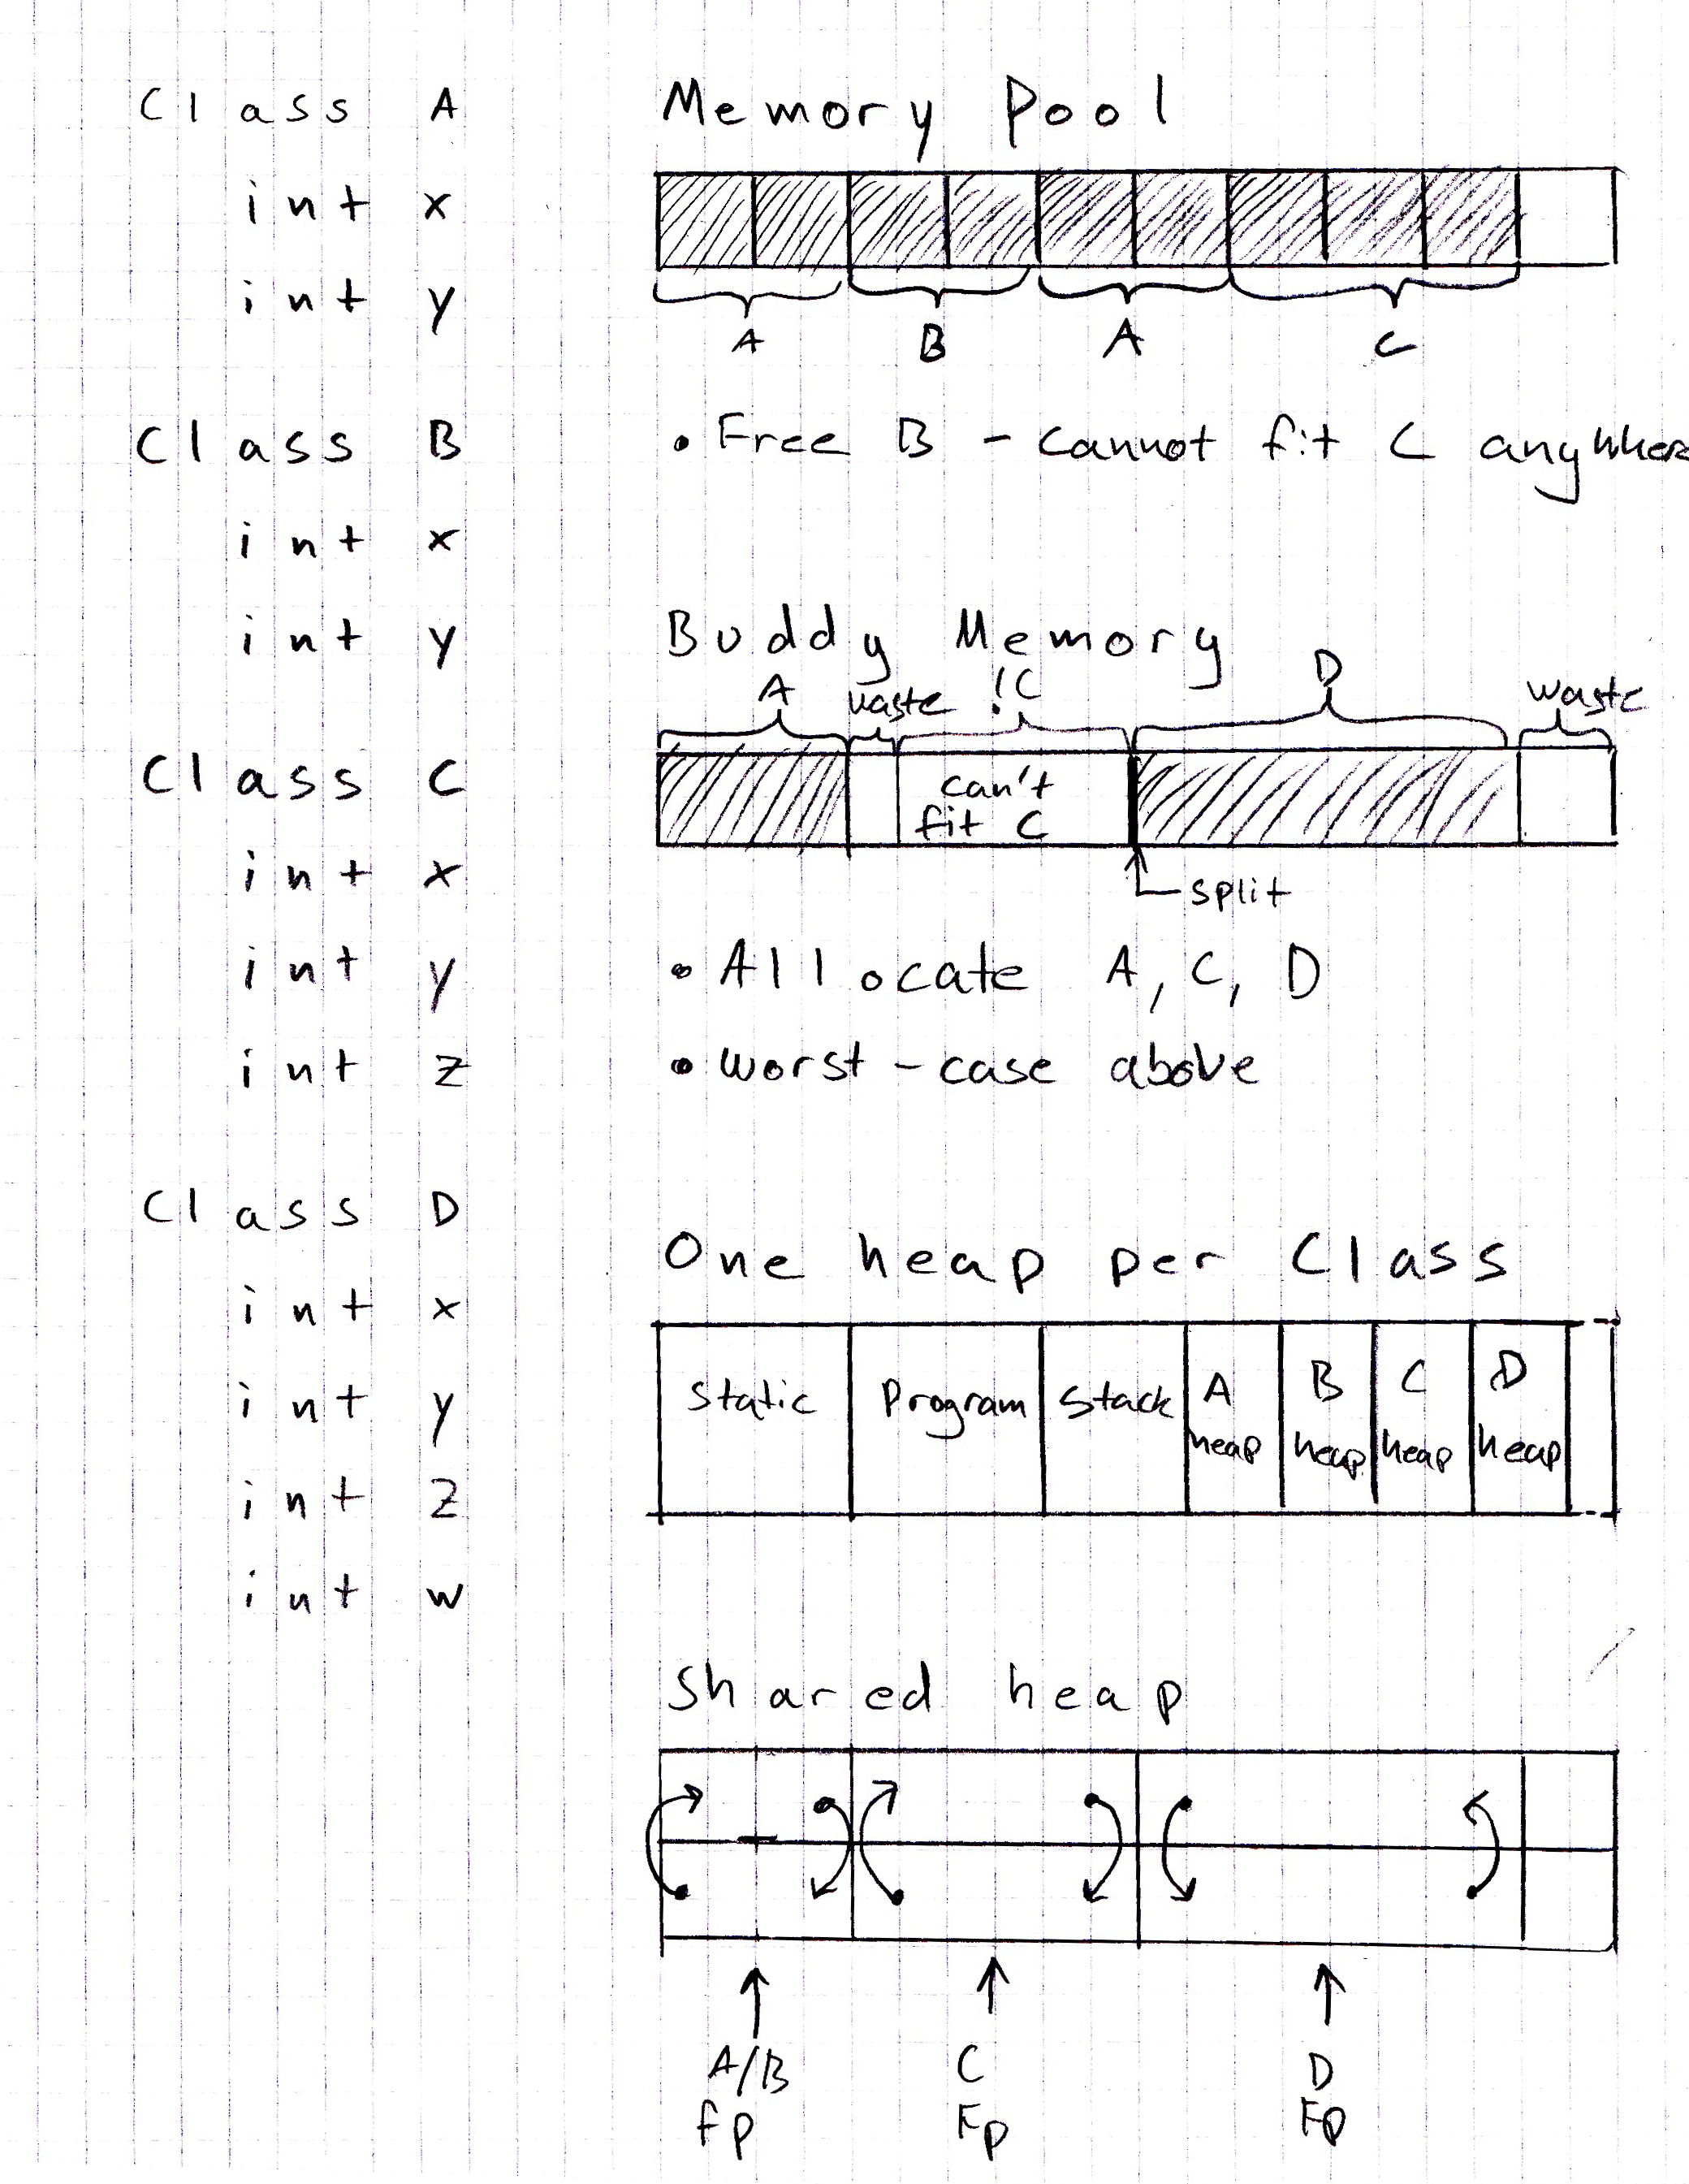
\includegraphics[width=0.7\textwidth]{heap-designs}
  \caption{Heap memory layouts (Draft)}
\end{figure}


\section{\rooplpp Memory Layout}
\label{sec:rooplpp-memory-layout}
\texttt{TBD}